\documentclass[8pt,a5paper, oldfontcommands]{memoir}

\usepackage[utf8]{inputenc}
\usepackage[english]{babel}

\usepackage{graphicx}
\usepackage{color}
\usepackage{float}
\usepackage{url}
\usepackage{listings}

\usepackage{microtype}
\setcounter{section}{0}

\hoffset = 10pt
%\voffset = -20pt

\usepackage{lipsum}

\renewcommand\thesection{\arabic{section}}

\begin{document}

\pagenumbering{gobble}% Remove page numbers (and reset to 1)
\clearpage
\thispagestyle{empty}

\begin{huge}
\textbf{Use of KFParticle with MPD}
\end{huge}

\begin{figure}[H]
  \centering
  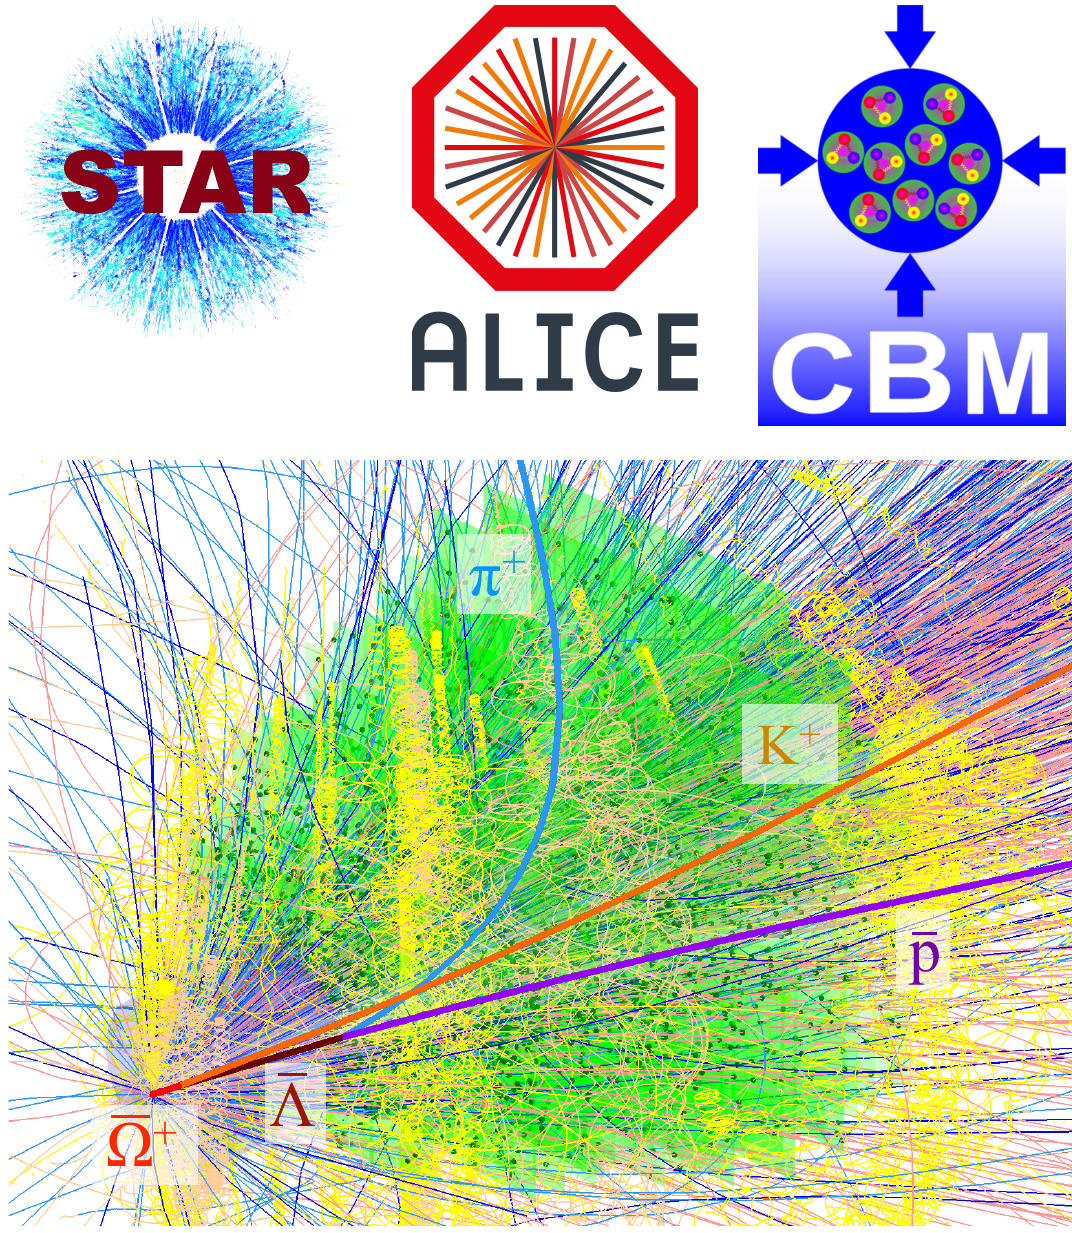
\includegraphics[width=0.5\textwidth]{img/particlesInCollision.png}
  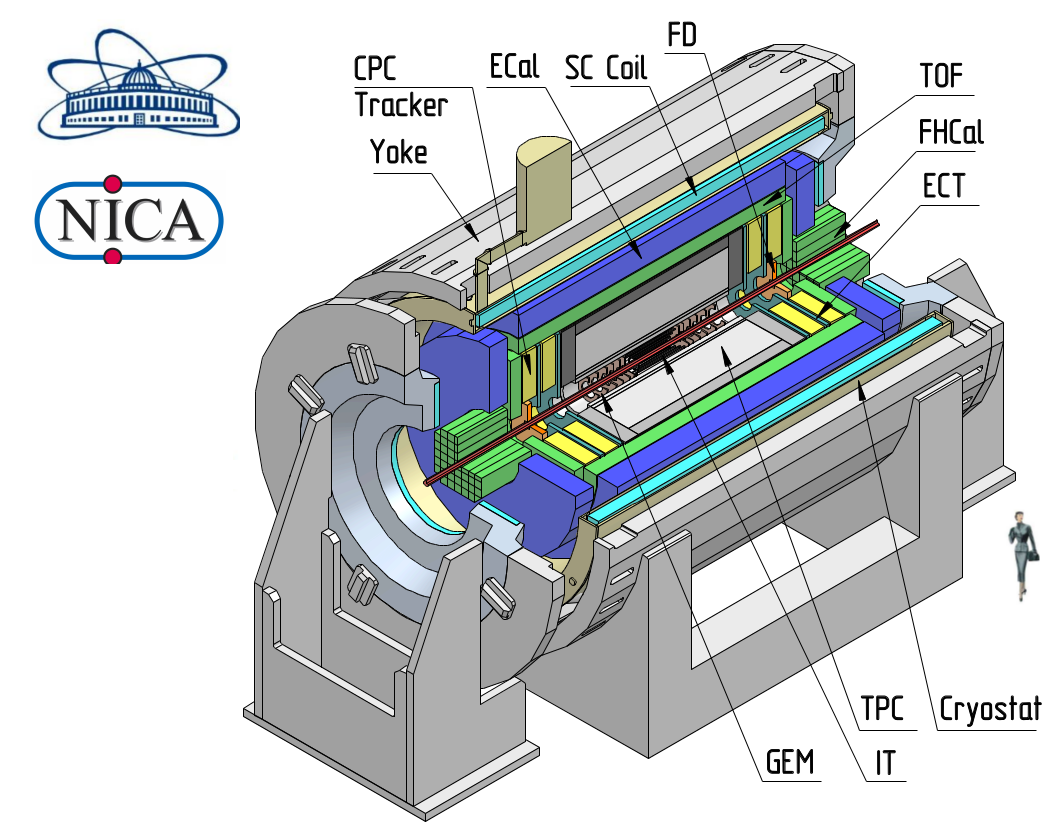
\includegraphics[width=0.5\textwidth]{img/mpd_addLogos.png}
\end{figure}

\begin{centering}
  \bf
  Contacts: \\
  Pavel Batyuk, VBLHEP, JINR, \url{pavel.batyuk@jinr.ru}
\end{centering}

\newpage

\pagenumbering{Roman}

\begin{normalsize}
\tableofcontents
\end{normalsize}

\newpage

\thispagestyle{plain}

\pagenumbering{arabic}

\section{Introduction}
\thispagestyle{plain}

KFParticle is a formalism specially developed for complete reconstruction of short-lived particles with their
momentum $P$, energy $E$, mass $m$, lifetime $c\tau$, decay length $L$ and so on.
Its main benefits are listed below:
\begin{itemize}
\item based on the Kalman filter mathematics idependent in sense of experimental setup (collider or fixed target)
\item allows one reconstruction of decay chains (cascades)
\item daughter and mother particles are described and considered the same way
\item daughter particles are added to the mother particle independently
\end{itemize}

At the moment, the power abilities of KFParticle can be used in the MpdRoot software. It is embedded into MpdRoot as a module with all necessary dependencies
and a first version of particle finder respectively to MPD that uses all the benefits by KFParticle, has been developed.
The manual has a goal to share experience on how to use the main macroses aiming at production of output with its subsequent analysis in user's codes.
It is not a finished job since the develpment (description) procedure is ongoing.  

\newpage
\section{How to produce output for analysis?}
\thispagestyle{plain}

Right now, the package has one main macro to be used for starting the software (namely, to produce output).

The macro can be found in the {\color{blue} macro/KFParticle/runKFParticle} directory of the MPD software.
It is called {\color{blue} runKFParticleFinder.C} (see below in p. 6).

It inherits all benefits from FairRoot to work in a ``task''-way mode processing passed events in chain.

There are two options how user can pass input data to the macro. The most trivial one is that one passes a single file written either
in the {\color{red} standard dst-format} or in the {\color{blue} MiniDst format}. The latter is fully supported by the software,
but one has to take into account that MiniDst input should be produced with a code version where there is a correct parameterization of covariance matrix used.
Looking at a "suitable'' file one sees the following parameterization of covariance matrix:

\begin{figure}[H]
  \centering
  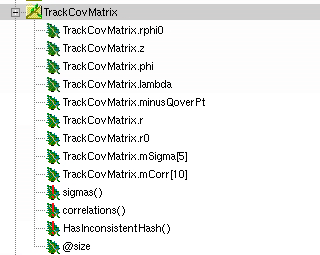
\includegraphics[width=0.4\textwidth]{img/covarMatrix.png}
  \caption{\bf Example how a correct parameterization of covariance matrix looks like}
\end{figure}

The second option how to provide input for the software looks more preferred since it works with a list of files. The passed list should have *.lis or *.list extension and the following format:

\begin{figure}[H]
  \centering
  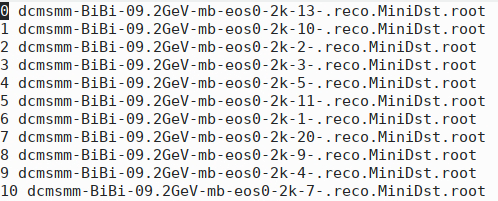
\includegraphics[width=0.5\textwidth]{img/exampleList.png}
  \caption{\bf Example of list (*.lis or *.list) to be passed to software}
\end{figure}

Each line contains a file identifier (file ID) and dst name (supported, surely, both formats as mentioned before). The identifier is considered to be obligatory since it allows one in subsequent analysis to get information on file name and, in particular, event number.
The list is limited by five thousand (5000) lines (e.g. files) to be put inside.

Also user should define an output file name and desirable number of events to process. The number of events in the case of a passed list means number of consecutive events
(from the total number of events passed in the list) aimed to be processed. If the number is equal to zero, it means that the whole dataset is assumed to be processed. 

The macro also instantiates the Kalman filter since it is used for doing extrapolation of track parameters to the inner TPC shell.

The main object of the software is called {\bf MpdKfParticleFinder} and represents itself a first {\bf version of particle finder approach based on the KFParticle formalism respectively to MPD}.
Generally speaking, it is an interface to KFParticle that takes into account important things how to work with existing reconstruction output from the detector (namely, TPC at the moment).
It does support of two existing dst formats in MPD and used track parameterization (see Fig.\ref{fig1}).
\begin{figure}[H]
  \centering
  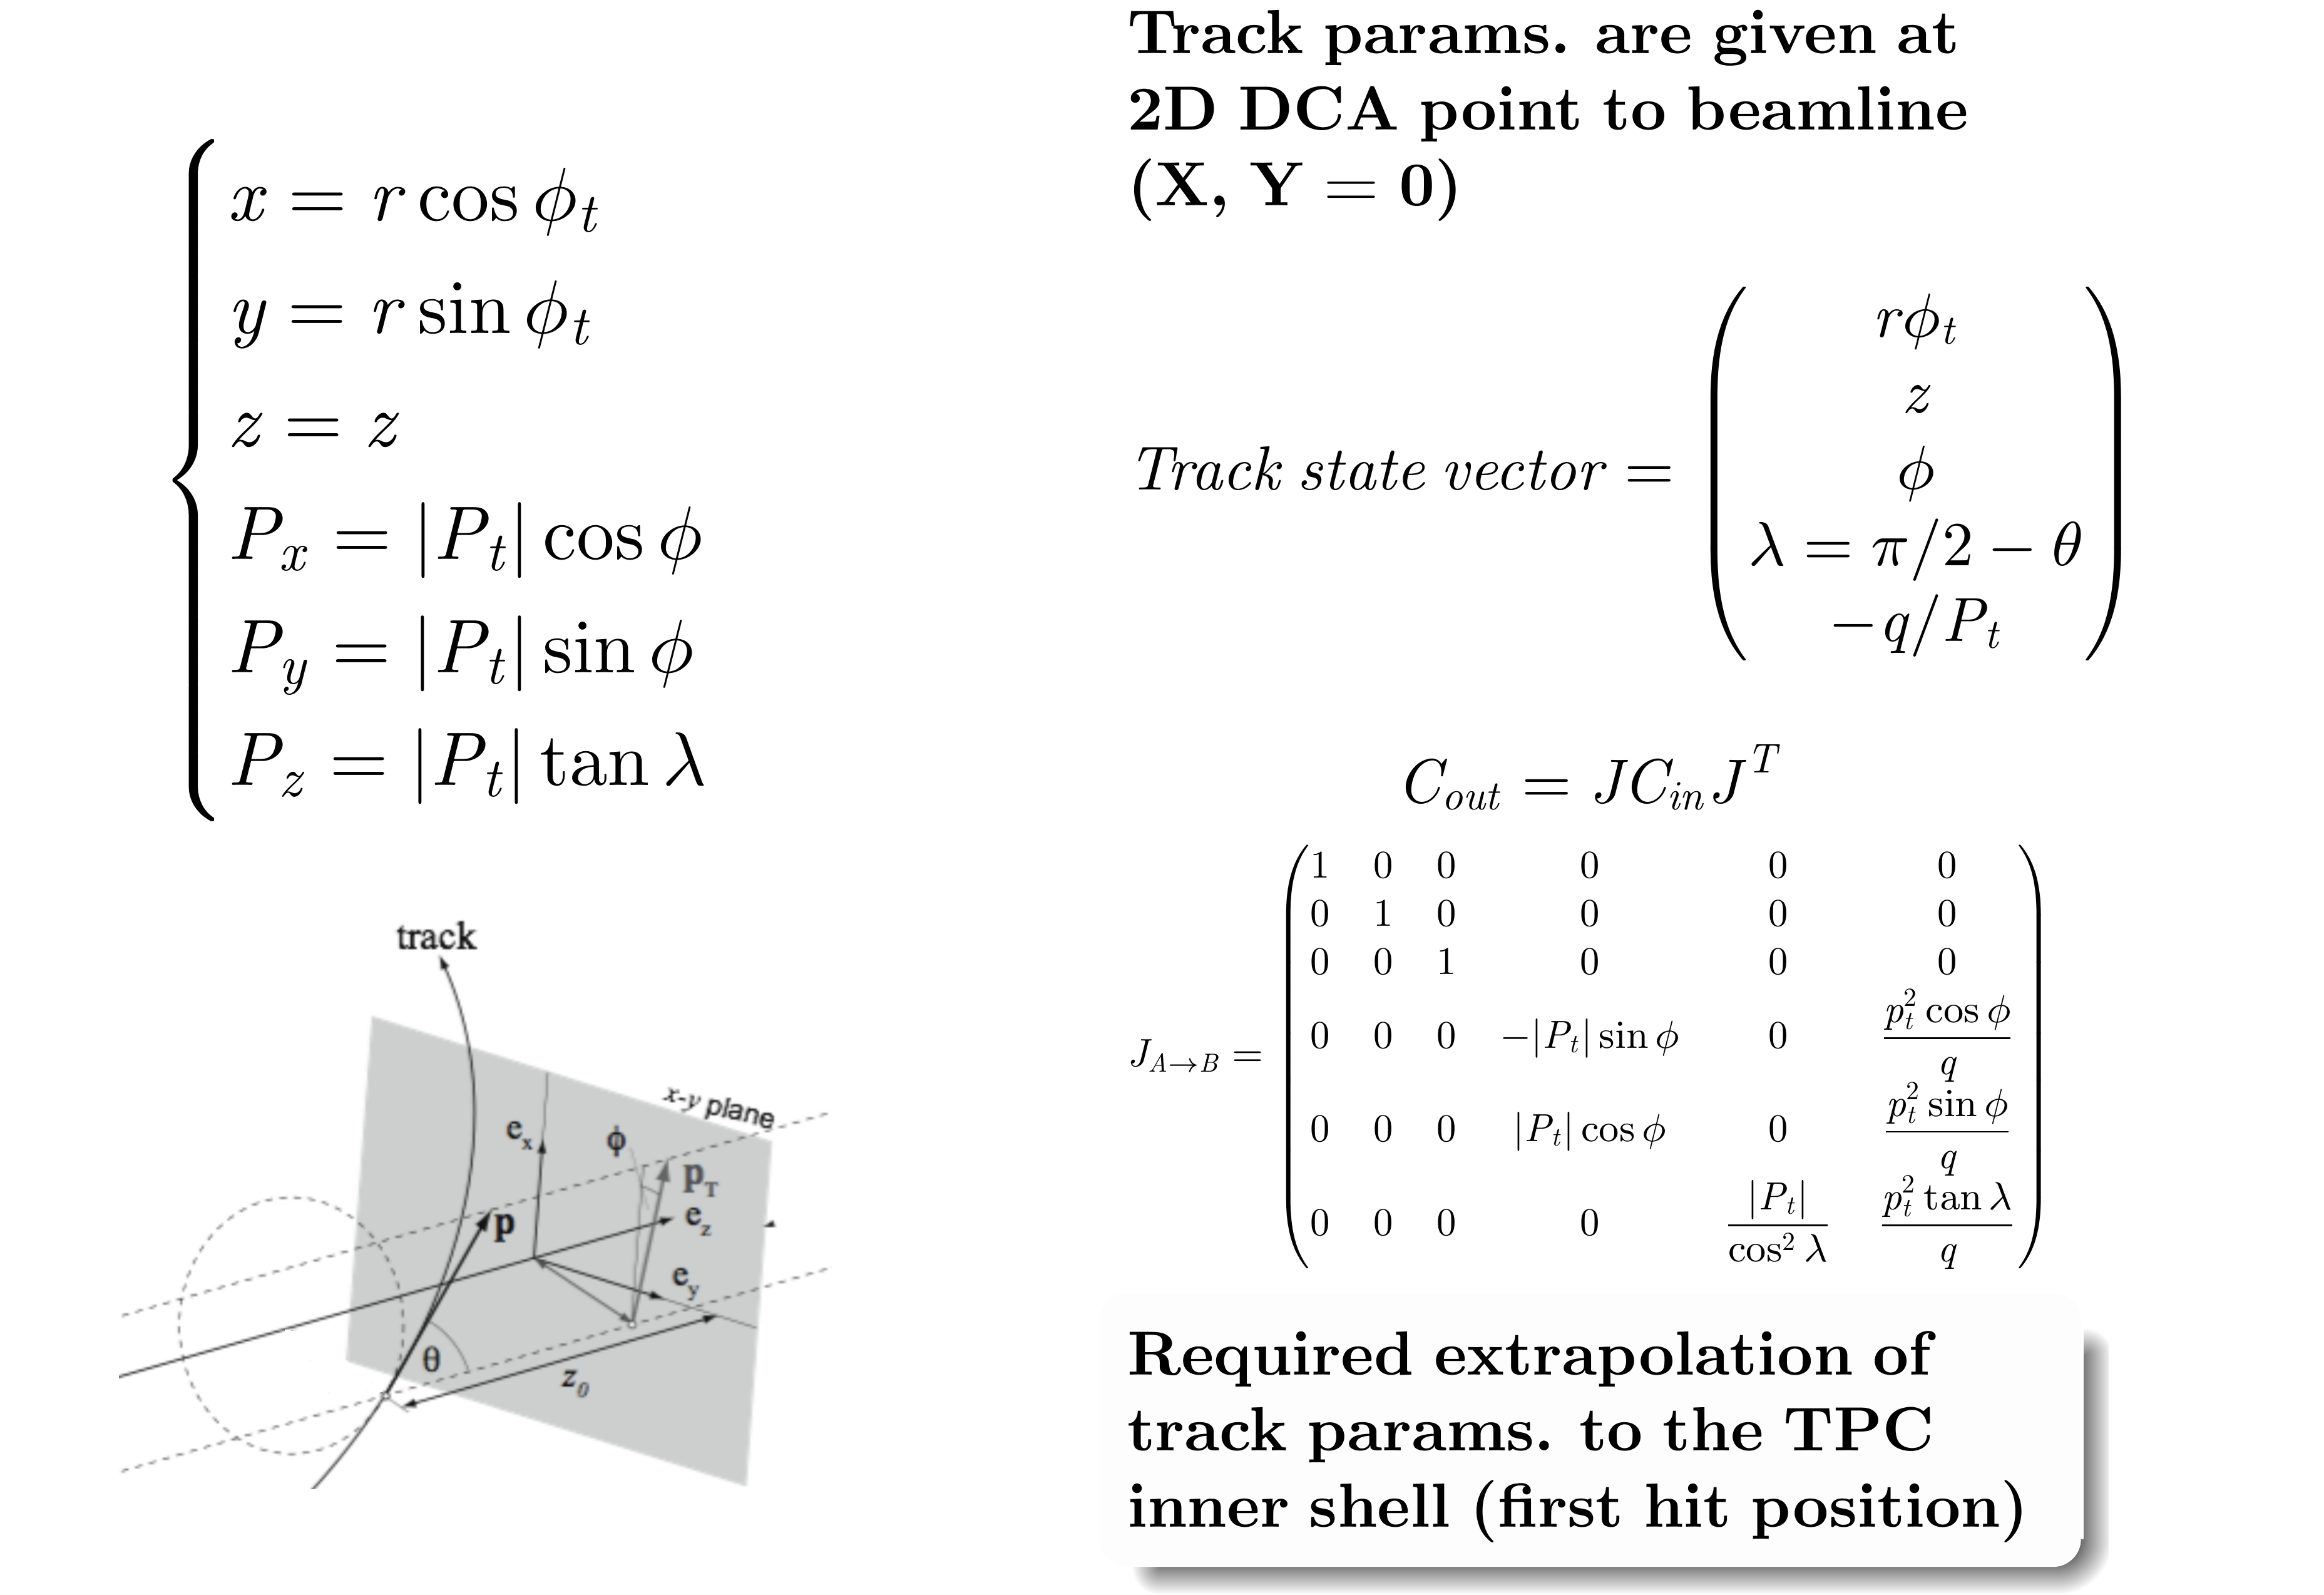
\includegraphics[width=0.6\textwidth]{img/trackParams.png}
  \caption{\bf Example of track parameterization in MPD}
  \label{fig1}
\end{figure}

The latter is the most important part of the particle finder.
Also, a simple mechanism to select input tracks with desirable kinematical characteristics (transverse momentum, rapidity) is realized.

A brief explanation of the main modificators to {\bf MpdKfParticleFinder} is given in the table. The modificators are set by default values in the software, but user has a possibility
to reset them if necessary.
 \begin{table}[H]
      % \resizebox{\columnwidth}{!}{%
         \begin{tabular}{|c|l|} 
           \hline
           Modifier & Explanation \\
           \hline
           \bf SetPidHypo(pdg1, pdg2) & {\color{blue} \bf Default values are 2212 and -211}\\
           & At the moment, it is possible to select \\
           & only one additional decay for analysis. \\
           & Setting (+211, -211) corresponds to \\
           & $K_{s}^{0} \rightarrow \pi^{+} + \pi^{-}$ \\
           & \color{red} \bf Temporary solution to change \\
           & \color{red} \bf in the future \\
           \hline
           \bf SetUseCuts(flag) & {\color{blue} \bf Default flag value is false.} \\
           & If set with true, it means that tracks \\
           & are chosen according to the established \\
           & values. The cuts are set by {\bf TrackCuts}. \\
           & At the moment, it is possible to define \\
           & values for pseudorapidity and transverse \\
           & momentum in sense of track acceptance.\\
           \hline
           \bf SetUseKFPerformance(flag) & {\color{blue} \bf Default flag value is false.} \\
           & Returning it to true gives opportunity \\
           & to produce QA histograms proposed by \\
           & KFParticle performance tools. \\ 
           & They seem to be very useful when \\
           & doing comparison between Monte Carlo \\
           & and reconstruction aiming at developing \\
           & cuts to suppress background and so on. \\
           & {\color{red} \bf Important note: it works just} \\
           & {\color{red} \bf with standard dst!!!} \\
           \hline
         \end{tabular}
       %}
 \end{table}



 \newpage
 \thispagestyle{plain}
{ \scriptsize
\begin{lstlisting}[language=C++,basicstyle=\ttfamily,keywordstyle=\color{red}, commentstyle=\color{blue}]
void runKFParticleFinder(TString in = "", TString out = "",
Int_t nStartEvent = 0, Int_t nEvents = 0) {
FairRunAna* fRun = new FairRunAna();
FairRootFileSink* sink = new FairRootFileSink(out);
fRun->SetSink(sink);

MpdKalmanFilter *kalman = MpdKalmanFilter::Instance("KF");
fRun->AddTask(kalman);

MpdKfParticleFinder* pF = new MpdKfParticleFinder(in);
// pF->SetUseCuts(kTRUE);
// pF->SetUseKFPerformance(kTRUE);
    
// Setters to specify what a two-particle decay we are looking for ... 
// pdg1, pdg2 to specify a decay. \Lambda^{0} is set by default
// Available decays right now are:
// \Lambda^{0} -> p + \pion^{-} and
// \Kaon^{0}_{s} -> \pion^{+} + \pion^{-}

// pF->SetPidHypo(+211, -211);
    
fRun->AddTask(pF);
fRun->Init();

// Redefine established cuts if necessary ...
//    TrackCuts* cutsGot = partFinder->GetTrackCuts();
//    if (cutsGot) {
//        cutsGot->SetPtMin(.5);
//        cutsGot->SetPtMax(1.8);
//        cutsGot->SetAbsEta(1.);
//    }

fRun->Run(nStartEvent, nStartEvent + nEvents);
    
delete pF;
} 
\end{lstlisting}
}

\newpage
\section{How to read produced output?}
\thispagestyle{plain}

To use a result of work of particle finder one is refferred to {\color{blue} readKFParticleOutput.C} located, evedently, in the macro/KFParticle directory.
The macro illustrates how to get output from the previous step and use it.

Besides of decaying particles to be reconstructed, the software is able to perform reconstruction of primary vertex ($V_{p}$) of interaction. In the most general case,
it allows (KFParticle) one to get more than one primary vertex reconstructed, but existing current setup of the software reconstructs one candidate to be primary vertex.
At the moment, multiple vertices are not allowed to be reconstructed (particle finder).

Below are given explanations for some parts of {\color{blue} readKFParticleOutput.C} considered to be useful for users in their analyses.

{ \footnotesize
\begin{lstlisting}[language=C++,basicstyle=\ttfamily,keywordstyle=\color{red}, commentstyle=\color{blue}]
...
  // Getting information on reco file and event used ...
  // id of file in the list processed by runKFParticle.C
  Int_t fileId = eventHeader->GetInputFileId();

  // current event that corresponds to the same event in reco output
  Int_t evNum = eventHeader->GetMCEntryNumber(); 
...
\end{lstlisting}
}
A couple of values {\color{blue} (fileId, evNum)} are important when linking output from the software to the source reconstructed data. {\color{blue} fileId} corresponds to those one
defined in the list of files passed for analysis. So, taking into account this pair, one is able to get event {\color{blue} (evNum)} with all information from the source.

Information on reconstructed primary vertex is written into output with {\color{red} KFVertex}
{ \tiny
\begin{lstlisting}[language=C++,basicstyle=\ttfamily,keywordstyle=\color{red}, commentstyle=\color{blue}]
  ...
// Getting reconstructed primary vertex in event ...
// In general case, here should be a loop since we are able to reconstruct 
// more than one primary vertex ...
// One vertes is set by default in macro/KFParticle/runKFParticleFinder.C 
// It means that primVertices->GetEntriesFast() is equal to 1

for (Int_t iVertex = 0; iVertex < primVertices->GetEntriesFast(); iVertex++) {
KFVertex* Vp = (KFVertex*) primVertices->UncheckedAt(iVertex);

// To get a list of all possible accessors to written data, please,
// look at KFParticle/KFParticle/KFVertex.h
            
Float_t* covMatrix = Vp->CovarianceMatrix();
            
// Getting components of reconstructed vertex ...
Double_t X = Vp->GetX();
Double_t Y = Vp->GetY();
Double_t Z = Vp->GetZ();
            
// X = Y = Z = 0. means that primary vertex
// has not been reconstructed in event ...
if (!X || !Y || !Z)
    continue;
            
Int_t nContributors = Vp->GetNContributors();
}
  ...
\end{lstlisting}
}

The most important information that can be derived from the vertex section is three-dimensional coordinates of reconstructed vertex, number of participants used for the vertex reconstruction and,
surely, covariance matrix of vertex fit. A full list of accessors to be used is available at {\color{red} \bf KFParticle/KFParticle/KFVertex.h}
All necessary brief explanations are given there directly in the code when describing accessors.

Reconstructed secondary candidates are written to output with a very widely and frequently used {\bf \color{red} KFParticle} inherited from the {\bf \color{red} KFParticleBase} class.

A cycle illustrating how to get information on reconstructed secondaries is given below.
To select candidates that, probably, are considered as particles we are interested in, one uses PDG hypothesis of interesting particle.
So, to get, for example, $\Lambda^{0}$ candidates one has to do as follows:

{ \tiny
  \begin{lstlisting}[language=C++,basicstyle=\ttfamily,keywordstyle=\color{red}, commentstyle=\color{blue}]
for (Int_t iSecondary = 0; iSecondary < recoSecondaries->GetEntriesFast(); iSecondary++) {
KFParticle* particle = (KFParticle*) recoSecondaries->UncheckedAt(iSecondary);
            
// To get a list of all possible accessors to written data, please,
// look at KFParticle/KFParticle/KFParticle.h and KFParticle/KFParticle/KFParticleBase.h
            
Int_t pdgHypo = particle->GetPDG();
if (pdgHypo != pdg)
   continue;
            
Double_t mass = particle->GetMass();

Double_t Px = particle->GetPx();
Double_t Py = particle->GetPy();
Double_t Pz = particle->GetPz();
            
Double_t pT = particle->GetPt();
Double_t eta = particle->GetEta();
}
    
  \end{lstlisting}
}

\thispagestyle{plain}
{\bf \color {red} KFParticle} has a lot of accessors to parameters of reconstructed secondaries. It is possible to get {\bf \color{blue} mass, projection of momentum, rapidity, decay length} and many other characteristics of found secondaries.
A full list of accessors with brief descriptions is given in {\bf \color{red} KFParticle/KFParticle/KFParticle.h} and {\bf \color{red} KFParticle/KFParticle/KFParticleBase.h}
The most useful of them are planned to be marked and explained in Section~\ref{sec} in the nearest future.

Another important option is related to possibility of getting indices of particles that form interesting decay channel of decaying particle.
It is illustrated below how to do it. The feature works correctly just in case of standard dst used, since this case (at the moment, MiniDst does not support it yet)
we are able to construct a full chain that allows one to pass through all necessary steps and, finally, to get index of mother particle to judge whether the found candidate is true or false
assuming to be a desirable decaying particle. 

{ \tiny
  \begin{lstlisting}[language=C++,basicstyle=\ttfamily,keywordstyle=\color{red}, commentstyle=\color{blue}]
// It is possible to get indices of reconstructed tracks in standard / MiniDst. 
// Doing it for standard dst, one can get source Monte Carlo track to check 
// whether its mother is a desirable decaying particle we are looking for ...
// (daughter id given by particle finder --> idx of reconstructed track --> 
// --> idx of corresponding MC track --> idx of mother particle)
// To do it, one has to link standard dst to the macro in an usual way 
// fileId and evNum are available to get corresponding file, event and arrays
// with reconstructed tracks 
                       
const Double_t massThresh = 0.025;
if (TMath::Abs(mass) < massThresh) {
   Int_t nDaugh = particle->NDaughters();
   vector <Int_t> daughters = particle->DaughterIds();

   for (Int_t iDaugh = 0; iDaugh < nDaugh; iDaugh++)
      cout << daughters[iDaugh] << " ";
   cout << endl;
}
  \end{lstlisting}
}

\newpage
\section{The most useful methods provided by {\bf \color{red} KFParticle} to be used in user's analysis}
\label{sec}
\thispagestyle{plain}
{\bf The section is planned to be filled with descriptions of useful methods on how to use them correctly in user's analysis.}

\end{document}
